\section{Experimental Analysis for Prediction Algorithms}
\label{sec:experiment design}

As discussed in Section 3, some algorithms are more appropriate in certain 
scenarios. To study these algorithmic differences, we have developed indoor 
and in-field experiments on an off-the-shelf wireless platform.
%Testbed and emulator Platform
To ensure the results are broadly applicable, we employ a Linux-based 
802.11 testbed~\cite{Openwrt}. The platform includes a Gateworks 2358 
motherboard with Ubiquiti XR series radios (XR9 at 900 MHz, XR2 at 2.4 GHz, 
XR5 at 5.2 GHz) as well as a DoodleLabs DL475 radio at 
450 MHz~\cite{Gateworks,Ubnt}.  Another instrument involved in the 
experimentation is an Azimuth ACE-MX channel emulator, allowing 
controllable propagation and fading characteristics with a broad range of 
industry-standard channel models from 450 MHz to 5.9 GHz~\cite{AzimuthACE}. 

%context information experiments
\subsection{In-lab Experiments for Radio Characterization}
\label{subsec:ichannel}
To establish an SNR to throughput relationship for the \emph{SNR-based 
Throughput Look-up Algorithm}, we use an experimental setup where two 
wireless nodes communicate across repeatable emulated channels generated 
by Azimuth ACE-MX channel emulator (Fig.~\ref{fig:in-door experiment}). For a given band and card, we measure
the throughput of a fully-backlogged UDP flow using the {\it iperf} 
traffic generator. We use constant attenuation over an idealized
channel condition (i.e., a bypass channel) and repeat the experiment to
produce various RSSI values.
Despite the same physical and media access layers of the radios, there are
slight differences in the throughput achieved per radio at the same attenuation
level.  Thus, we normalize these throughput values to have the same maximum
throughput across radio types for a fair comparison of the frequency bands.

\begin{figure}
\vspace{-0.1in}
\centering
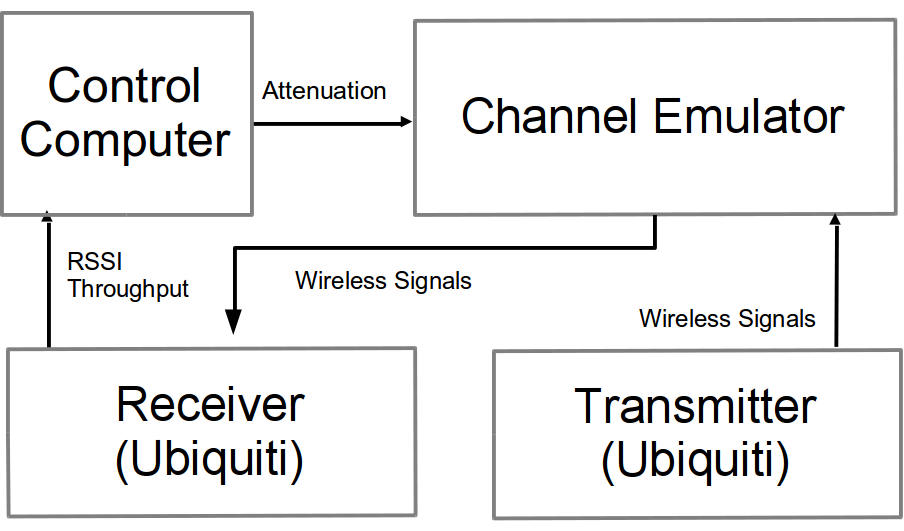
\includegraphics[width=65mm]{figure/emulator2}
\vspace{-0.1in}
\caption{Experimental setup for channel emulator.}
\label{fig:in-door experiment}
%\vspace{-0.1in}
\end{figure}

%\subsection{Signal Level Context-aware information}
\subsection{Experimental Design for In-field Data Collection}
\label{subsec:insitu}
We now describe the in-field experimental design to obtain a data set for
evaluating our multiband algorithms. Two Gateworks boards, each containing
the aforementioned four radios are installed on two cars.  One node is always
the receiver and at a fixed location. The other node is always the 
transmitter and traverses
around the block of a public park as shown in Figure~\ref{fig:infield},
one loop of which will be used as a unit of training in the next section.
 
\begin{figure}
%\vspace{-0.1in}
\centering
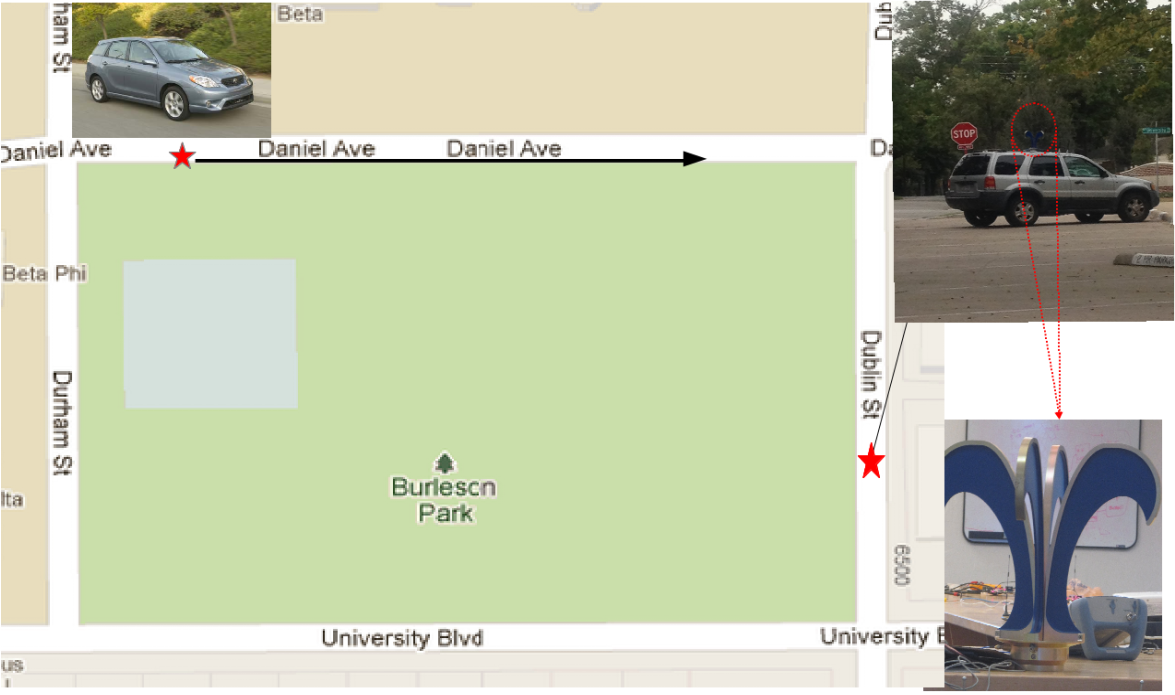
\includegraphics[width=75mm]{figure/infield}
\vspace{-0.1in}
\caption{In-field Experiment Setup}
\label{fig:infield}
\vspace{-0.1in}
\end{figure}

During each loop, the transmitter sends a fully-backlogged UDP flow
using {\it iperf} over each of the four radios simultaneously.  To
focus on band selection, we disable autorate and use a fixed data rate
of 6 Mbps. The receiver continually performs a {\it tcpdump} of all
received 802.11 packets~\cite{jacobson1989tcpdump}. Additionally, a
QH 400 Quad Ridge Horn antenna (shown in Figure~\ref{fig:infield}) is 
connected to a Rhode \& Schwarz FSH8 mobile spectrum analyzer at the 
receiver's location to monitor spectral activity. Then, based on the 
time stamps, 802.11 packets can be removed from the spectral trace 
so that only non-802.11 interference will contribute to $P_N^N$ for 
our algorithms.

\begin{figure}
\vspace{-0.1in}
\centering
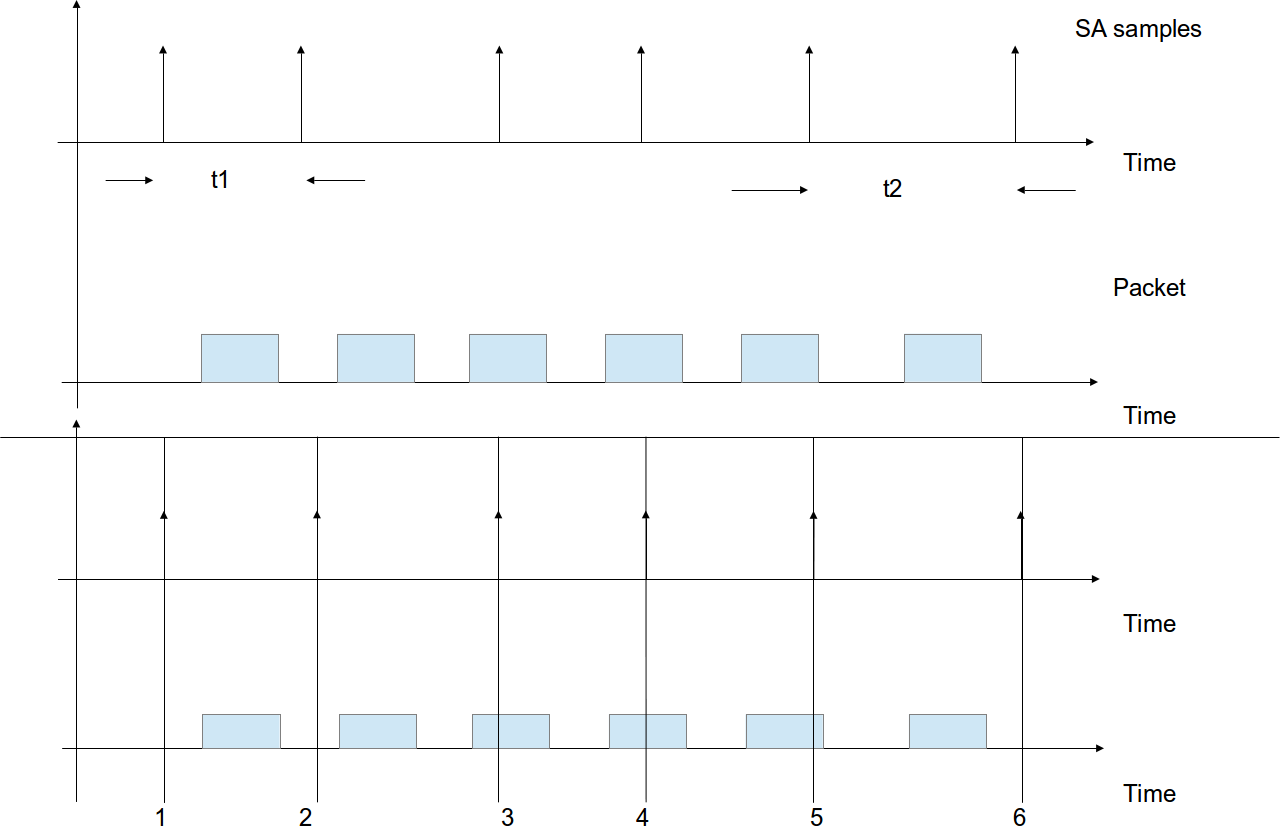
\includegraphics[width=65mm]{figure/sa_process}
\vspace{-0.1in}
\caption{Spectrum Analyzer Data Processing}
\label{fig:sa_process}
%\vspace{-0.1in}
\end{figure}

Figure~\ref{fig:sa_process} shows how we find the value of the
non-802.11 interference, $P_N^N$. We delete the spectrum analyzer
(SA) samples which overlap in time with the dumped 802.11 packets,
such as packet 3, 4, and 5 shown. Then, the reported interference value
will not contain received power from 802.11 packets which have already
been considered in the busy time, $B$.

The in-field data is processed offline where data from all instruments
involved is synchronized based on the GPS time stamps of each. 
As discussed in~\ref{subsec:ichannel}, the throughput of each radio
is normalized based upon the emulator experiment to account for any
manufacturing differences.

